\documentclass[aspectratio=169]{beamer}

%\documentclass{beamer}
\mode<presentation> {
\usetheme{Singapore}
\usefonttheme{default}
\usecolortheme{rose}
\setbeamertemplate{headline}
 {%
  \insertsectionnavigationhorizontal{\textwidth}{}{}
}


\setbeamertemplate{footline}[page number]% To replace the footer line in all slides with a simple slide count uncomment this line
\setbeamertemplate{navigation symbols}{} % To remove the navigation symbols from the bottom of all slides uncomment this line
}


\usepackage[export]{adjustbox}
\usepackage{bibentry}
\usepackage{graphicx} % Allows including images
\usepackage{booktabs} % Allows the use of \toprule, \midrule and \bottomrule in tables
\usepackage{caption}
\setbeamertemplate{caption}[numbered] % used to remove caption number
\usepackage{natbib}
\renewcommand{\bibsection}{\subsubsection*{\bibname }}
\usepackage[utf8]{inputenc}
\DeclareUnicodeCharacter{2010}{-}%
\usepackage{subfigure}
\usepackage{amssymb,amsmath}
\usepackage{amsthm}
\usepackage{graphicx}
\usepackage{tikz}
\usepackage{color}
\usetikzlibrary{positioning,shapes,arrows,snakes}
\usetikzlibrary{decorations.markings,calc,arrows.meta,snakes,decorations.pathmorphing, decorations.text}
\usepackage{animate}
\usetikzlibrary{arrows.meta}
\usetikzlibrary{calc}
\usetikzlibrary{external}
\tikzexternalize[prefix=Fig/tikz/]
\usepackage{pgfplots}
\usetikzlibrary{shapes}
\usepackage{epstopdf}
\setbeamerfont{frametitle}{size=\huge}
\usepackage{fancybox}
\usepackage{bm}
\usepackage{mathrsfs}
\everymath{\displaystyle}


\newcommand{\lb}{\raisebox{2pt}{%
\tikzset{external/export=false}%
\tikz{\draw[-,solid,line width = 1pt,color=black](0,0) -- (5mm,0);}}}

\newcommand{\lr}{\raisebox{2pt}{%
\tikzset{external/export=false}%
\tikz{\draw[-,solid,line width = 1pt,color=red](0,0) -- (5mm,0);}}}

\newcommand{\lc}{\raisebox{2pt}{%
\tikzset{external/export=false}%
\tikz{\draw[-,solid,line width = 1pt,color=cyan](0,0) -- (5mm,0);}}}

\newcommand{\lm}{\raisebox{2pt}{%
\tikzset{external/export=false}%
\tikz{\draw[-,solid,line width = 1pt,color=magenta](0,0) -- (5mm,0);}}}

\newcommand{\emphI}[1]{\textbf{\Large#1}}

%----------------------------------------------------------------------------------------
% Front page information
%----------------------------------------------------------------------------------------

\title{\huge Effects of fractures on seismic wave-fields in the presence of
equant porosity.} % The short title appears at the bottom of every slide, the full title is only on the title page

\author[Yuriy Ivanov]{\Large Yuriy Ivanov$^\text{1}$*, Giorgos Papagiorgiou$^\text{1,2}$,\\Alexey Stovas$^\text{1}$, Mark Chapman$^\text{2}$}
\institute{
$^\text{1}$Norwegian University of Science and Technology\\
$^\text{2}$The University of Edinburgh}
\date{
	\begin{columns}
		\begin{column}{0.25\textwidth}
  			\begin{center}
				
\includegraphics[width=1.5cm]{./Fig/ntnulogoengC}
			\end{center}
		\end{column}
		%
		\begin{column}{0.45\textwidth}
  			\begin{center}
				\large June 4th, 2019 \\ 81st EAGE Conference \& Exhibition
			\end{center}
		\end{column}
		%
		\begin{column}{0.25\textwidth}
  			\begin{center}
				
\includegraphics[width=1.5cm]{./Fig/eage}
			\end{center}
		\end{column}
\end{columns}
	}



%----------------------------------------------------------------------------------------
%	Footer
%----------------------------------------------------------------------------------------
\makeatletter
\setbeamertemplate{footline}
{
  \leavevmode%
  \hbox{%
   \begin{beamercolorbox}[wd=\paperwidth,ht=2.25ex,dp=2ex,center]{}
    \insertframenumber{} of \inserttotalframenumber{}
  \end{beamercolorbox}}%
  \vskip0pt%
}
\makeatother
%----------------------------------------------------------------------------------------
\newcommand\titleslide[1]{
	\begin{frame}
		\Huge
		\centering
		#1
	\end{frame}
	}
\begin{document}

\newcommand{\solid}{\raisebox{2pt}{\tikz{\draw[-,solid,line width = 1pt](0,0) -- (5mm,0);}}}

\newcommand{\dashed}{\raisebox{2pt}{\tikz{\draw[-,dashed,line width = 1pt](0,0) -- (5mm,0);}}}




\tikzset{>=Stealth}
{\setbeamertemplate{footline}{} % removes footer from the front page
\begin{frame}
	\titlepage
\end{frame}
}

%----------------------------------------------------------------------------------------
%	PRESENTATION SLIDES
%----------------------------------------------------------------------------------------
\begin{frame}
\frametitle{Outline}
\tableofcontents 
\end{frame}
%------------------------------------------------
\section[Introduction]{Introduction}
%------------------------------------------------
\titleslide{Introduction}
%------------------------------------------------
\begin{frame}{Motivation}
\centering
\tikzset{external/export=false}
	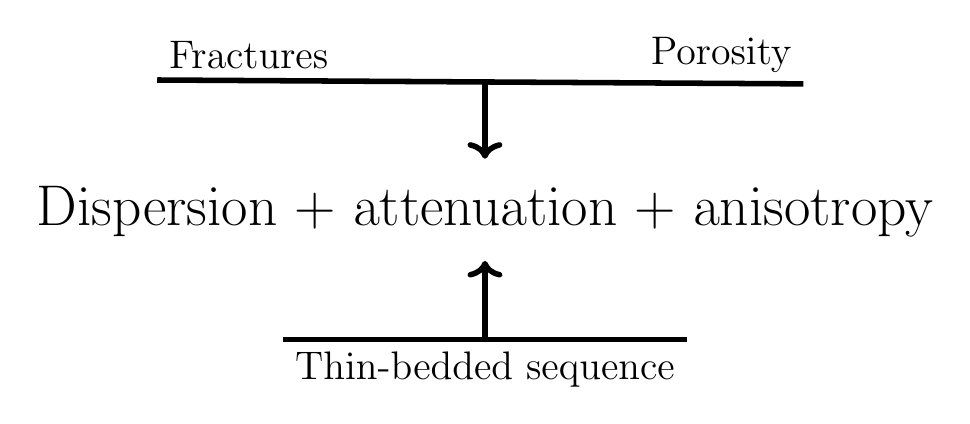
\begin{tikzpicture}[line width=2pt]
		\node[] at (0,-2) {\huge Dispersion + attenuation + anisotropy};
		
		\onslide<2->{
		\node[] (F) at (-3,0) {\Large Fractures};
		\node[] (P) at (3,0) {\Large Porosity};
		\draw[] (F.south west) -- (P.south east);
		\node[] (O) at (0,0) {\Large \vphantom{FOO}};
		\draw[-To] (O.south) --++ (0,-1);
		}
		
		\onslide<3->{
		\node[] (TL) at (0,-4) {\Large Thin-bedded sequence};
		\draw[] (TL.north west) -- (TL.north east);
		\draw[-To] (TL.north) --++ (0,1);
		}
	\end{tikzpicture}
\end{frame}
%------------------------------------------------
\begin{frame}{Motivation}
\large \centering
Combine the \emphI{full-wavefield anisotropic modelling}
\\[1.5em]\pause
with the \emphI{rock-physics model of \citet{chapman_frequency-dependent_2003}}
\\[1.5em]\pause
to study how the \emphI{fracture length} affects
\\[1.5em]
the \emphI{wavefiled}
\\[1.5em]\pause
in the presence of \emphI{equant porosity}.
\end{frame}
%------------------------------------------------
\section[Reflectivity modeling]{Reflectivity modeling}
%------------------------------------------------
\titleslide{Reflectivity modeling}
%------------------------------------------------
\begin{frame}{Model: unbounded stack of layers}
\centering
	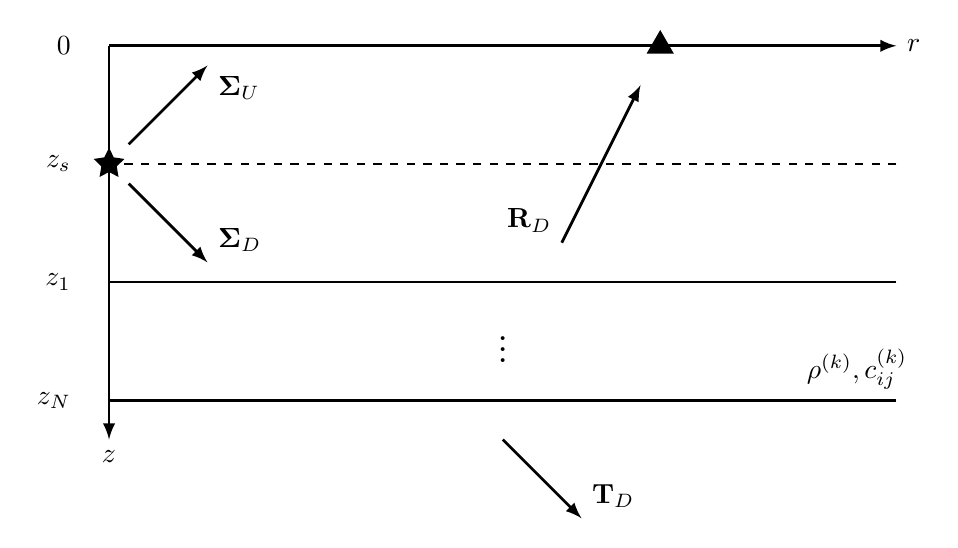
\begin{tikzpicture}[line width=1]
		\def\h{5}
		\def\l{10}
		\def\zs{1.5}
		\def\zb{3}
		\def\zN{4.5}
		\def\r{7}
		\draw[-latex] (0,\h) -- (0,0) node[below] {$z$};
		\node[left] at (0,\h) {$0\quad$};
		\draw[-latex] (0,\h) -- (\l,\h) node[right] {$r$};
		\draw[dashed] (\l,\h-\zs) -- (0,\h-\zs) node[left] {$z_s\quad$};
		\draw[] (\l,\h-\zb) -- (0,\h-\zb) node[left] {$z_1\quad$};
		\draw[] (\l,\h-\zN) -- (0,\h-\zN) node[left] {$z_N\quad$};
		\node[] at (\l/2,{\h-\zN+(-\zb+\zN)/2}) {\Large$\vdots$};
		\node[star,star points=3,star point ratio=0.5,draw,fill=white,fill=black,rotate=180] (R) at (\r,\h) {};
		\node[star,star points=5,star point ratio=0.5,draw,fill=white,fill=black,rotate=180] (S) at (0,\h-\zs) {};
		
		\draw[-latex] (S) ++(.25,-.25) --++ (1,-1) node [anchor=south west] {$\mathbf{\Sigma}_D$};
		\draw[-latex] (S) ++(.25,.25) --++ (1,1) node [anchor=north west] {$\mathbf{\Sigma}_U$};
		\draw[latex-] (R) ++(-.25,-.5) --++ (-1,-2) node [anchor=south east] {$\mathbf{R}_D$};
		\draw[-latex] (S) ++(\l/2,-\h+\zs) --++ (1,-1) node [anchor=south west] {$\mathbf{T}_D$};
		\node[anchor=south] at (\l-.5,\h-\zN) {$\rho^{(k)},c_{ij}^{(k)}$};
	\end{tikzpicture}
\end{frame}
%------------------------------------------------
\begin{frame}{Equations: P-SV system}\Large
	Equation of motion in $t-x$ domain:
	\begin{equation}
		\rho \frac{\partial^2 u_i}{\partial t^2} = \frac{\partial \sigma_{ij}}{\partial x_j} + f_i.
	\end{equation}
	Consecutive equation (Hooke's law):
	\begin{equation}
		\sigma_{ij} = \frac{1}{2} c_{ijkl} \left(\frac{\partial u_k}{\partial x_l} + \frac{\partial u_l}{\partial x_k}\right).
	\end{equation}
\end{frame}
%------------------------------------------------
\begin{frame}{Equations: Fourier-Bessel transform}\Large
	\begin{equation}
		F(k,\omega) = \mathscr{F}_\nu (f) = \int\limits_{-\infty}^{\infty} dt e^{i \omega t}\int\limits_{0}^{\infty} dr r J_\nu (kr) f(r,t),
	\end{equation}
	where $\nu=0,1$.
\end{frame}
%------------------------------------------------
\begin{frame}{Equations: P-SV system}\Large
	Wave equation in $\omega-k$ domain (post Fourier-Hankel transform $\mathscr{F}$):
	\begin{equation}
		\frac{d \mathbf{b}}{dz} = \omega \begin{bmatrix} 0 & \mathbf{A} \\ \mathbf{B} & 0 \end{bmatrix} \mathbf{b} {\color<2>{white}+ \mathbf{F}},
	\end{equation}
	where
	$$
		\mathbf{b} = \left[ \omega U_z, -S_r, S_Z, \omega U_r  \right]^T,
	$$
	and
	$$
		U_r, S_r = \mathscr{F}_1 (u_r,\sigma_{zr}), \quad U_z, S_z = \mathscr{F}_0 (u_z,\sigma_{zz})
	$$
\end{frame}
%------------------------------------------------
\begin{frame}{Equations: wavefields separation}\Large
	Up/down wavefield separation:
	\begin{equation}
		\mathbf{b} = \mathbf{L} \begin{bmatrix}\mathbf{u}\\\mathbf{d}\end{bmatrix},
	\end{equation}
	where $\mathbf{L}=\mathbf{L}(p,\omega,\rho,c_{ij})$, and $\mathbf{W}=\begin{bmatrix}\mathbf{u}\\\mathbf{d}\end{bmatrix}$ is the wave vector.
\end{frame}
%------------------------------------------------
\begin{frame}{Equations: reflectivity recursion}\Large
	Reflectivity response of the stack then:
	\begin{equation}\begin{aligned}
		\mathbf{R}_D(z_{j-1}|z_N) = \mathbf{E}_j\big\{\mathbf{R}_{D_j}+&\mathbf{T}_{U_j}\mathbf{R}_D(z_j|z_N)\times\\&\left[\mathbf{I}+\mathbf{R}_{D_j}\mathbf{R}_D(z_j|z_N)\right]^{-1}\mathbf{T}_{D_j}\big\}\mathbf{E}_j,
	\end{aligned}\end{equation}
	where
	$\mathbf{E}_j=\exp\left(i \omega \mathbf{q} z_j\right)$ and $\mathbf{q}=\text{diag} \left(q_\alpha,q_\beta\right)$.
\end{frame}
%------------------------------------------------
\begin{frame}{Equations: response of a point source}\Large
	Up-going wavefield at $z=0$ (no free surface) \citep{ursin_review_1983}:
	\begin{equation}
		\mathbf{U}(z_0) = \mathbf{R}_D(z_0) \mathbf{S}_2 - \mathbf{S}_1,
	\end{equation}
	where
	\begin{equation}
		\mathbf{S} = \mathbf{Q}(z_0|z_s) \mathbf{\Sigma}(z_s) = \begin{bmatrix}\mathbf{S}_1\\\mathbf{S}_2\end{bmatrix},
	\end{equation}
	and
	$\mathbf{Q}=
	\begin{bmatrix}
	\exp\left(i \omega \mathbf{q} z_s\right) &\\
	& \exp\left(-i \omega \mathbf{q} z_s\right)	
	\end{bmatrix}$.
\end{frame}
%------------------------------------------------
\begin{frame}{Equations: source vector}\Large
	Source is included as a wave-vector discontinuity \citep{kennett_seismic_2009}:
	\begin{equation}
		\left[\mathbf{W}(z_s)\right]^\pm=\mathbf{\Sigma}(z_s) = \begin{bmatrix}\mathbf{\Sigma}_U(z_s)\\\mathbf{\Sigma}_D(z_s)\end{bmatrix}.
	\end{equation}
	Alternatively, a stress-displacement vector discontinuity
	\begin{equation}
		\mathbf{\Sigma}(z_s) = \mathbf{L}^{-1} \left[\mathbf{b}\right]^\pm=\mathbf{L}^{-1}\mathbf{F}.
	\end{equation}
\end{frame}
%------------------------------------------------
\titleslide{Rock-physics model}
%------------------------------------------------
\section{Rock-physics model}
%------------------------------------------------
\begin{frame}{Rock-physics model\footnote{\citet{chapman_frequency-dependent_2003}}}
	\centering
	\tikzset{external/export=false}
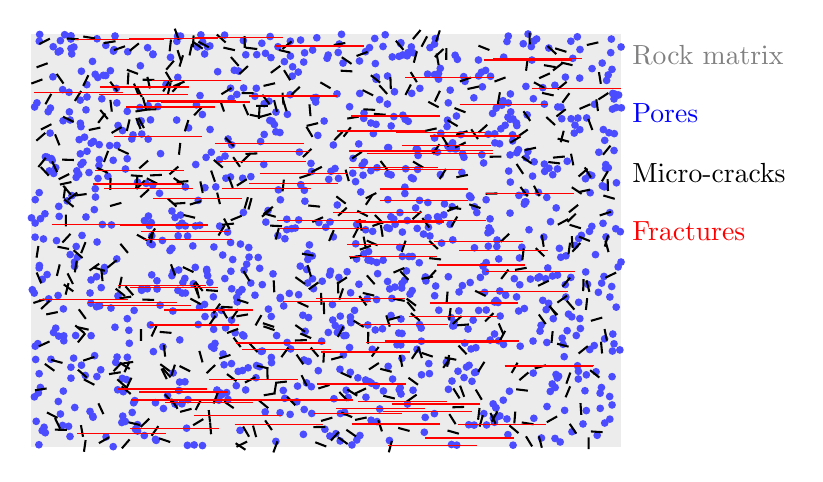
\begin{tikzpicture}[scale=0.75,line width=1.25]
		\def\l{10}
		\def\h{7}
		\def\Nf{100}
		\def\Nmc{500}
		\def\Np{1000}
		\def\fraclen{1.5}
		\def\mcracklen{\fraclen/7.5}
		\pgfmathsetseed{42}
		
		\fill [gray!15!white] (0,0) rectangle ++(\l,\h);

		\onslide<2->{
    		% pores
    		\foreach \i in {1,...,\Np}{
    			\pgfmathsetmacro\xi{\l*rnd}
    			\pgfmathsetmacro\yi{\h*rnd}
    				\draw[line width=.5pt,blue!70!white,fill=blue!70!white] (\xi,\yi) circle (1.5pt);
    				}
		}
		
		\onslide<3->{
    		%micro-cracks
    		\foreach \i in {1,...,\Nmc}{
    			\pgfmathsetmacro\xi{(\l-\mcracklen)*rnd+\mcracklen/2}
    			\pgfmathsetmacro\yi{\h*rnd}
			\pgfmathsetmacro\ai{180*rnd}
    				\draw[line width=.75,color=black, rotate around={\ai:(\xi,\yi)}] (\xi,\yi) ++ (-\mcracklen/2,0) --++ (\mcracklen,0);
    				}
    		}
		
    		\onslide<4->{
    		%fractures
    		\foreach \i in {1,...,\Nf}{
    			\pgfmathsetmacro\xi{(\l-\fraclen)*rnd+\fraclen/2}
    			\pgfmathsetmacro\yi{\h*rnd}
    				\draw[line width=.5,color=red] (\xi,\yi) ++ (-\fraclen/2,0) --++ (\fraclen,0);
    				}
    		}
					
		\node[anchor=north west] (RM) at (\l,\h) {\color{gray} Rock matrix};

		\onslide<2->{
		\node[anchor=north west] (RM) at (\l,\h-1) {\color{blue} Pores};
		}
		\onslide<3->{
		\node[anchor=north west] (RM) at (\l,\h-2) {\color{black} Micro-cracks};
		}
		\onslide<4->{
		\node[anchor=north west] (RM) at (\l,\h-3) {\color{red} Fractures};
		}
	\end{tikzpicture}
\end{frame}
%------------------------------------------------
\begin{frame}{Rock-physics model}{Dispersion}\Large\centering
\begin{tabular}{@{}lcl@{}}
	\color{gray}$\lambda = 10.69$ GPa		&&\color{gray}$\mu$ = 21.97 GPa\\
	\color{gray}$\rho$ = $2.15$ g/cc 		&& \\[.5em] \pause
	\color{blue}$\phi= 28$ \%				&&\color{blue}$\kappa_f$ = 2.4 GPa\\
	\color{blue}$r_{pores}$ = $10^{-4}$ m	&&\color{blue}$\tau_m$ = 2$\times10^{-5}$ s\\[.5em] \pause
	\color{black}$\varepsilon$ = 2 \%		&&$a_{mc}$ = 10$^{-5}$\\[.5em] \pause
	\color{red}$\varepsilon_f$ = 3 \%		&&\color{red}$L=\{1, 2, 3\} \times 10^{2} \times r_{pores}$
\end{tabular}
\end{frame}
%------------------------------------------------
\begin{frame}{Rock-physics model}{Dispersion}\Large\centering
	\includegraphics<1>[width=.45\textwidth]{./Fig/vel-P}%
	\includegraphics<2>[width=.45\textwidth]{./Fig/vel-P1}%
	\includegraphics<3>[width=.45\textwidth]{./Fig/vel-P2}%
	\includegraphics<4>[width=.45\textwidth]{./Fig/vel-P3}%
	\includegraphics<5>[width=.45\textwidth]{./Fig/vel-P4}%
	\quad%
	\includegraphics<1>[width=.45\textwidth]{./Fig/vel-S}%
	\includegraphics<2>[width=.45\textwidth]{./Fig/vel-S1}%
	\includegraphics<3>[width=.45\textwidth]{./Fig/vel-S2}%
	\includegraphics<4>[width=.45\textwidth]{./Fig/vel-S3}%
	\includegraphics<5>[width=.45\textwidth]{./Fig/vel-S4}%
	\\%
	$L$ = 0 (\lb), $L$ = 100 (\lr), $L$ = 200 (\lc), $L$ = 300 (\lm)
\end{frame}
%------------------------------------------------
\begin{frame}{Rock-physics model}{Attenuation}\Large\centering
	\includegraphics<1>[width=.45\textwidth]{./Fig/q-P}%
	\includegraphics<2>[width=.45\textwidth]{./Fig/q-P1}%
	\includegraphics<3>[width=.45\textwidth]{./Fig/q-P2}%
	\includegraphics<4>[width=.45\textwidth]{./Fig/q-P3}%
	\includegraphics<5>[width=.45\textwidth]{./Fig/q-P4}%
	\quad%
	\includegraphics<1>[width=.45\textwidth]{./Fig/q-S}%
	\includegraphics<2>[width=.45\textwidth]{./Fig/q-S1}%
	\includegraphics<3>[width=.45\textwidth]{./Fig/q-S2}%
	\includegraphics<4>[width=.45\textwidth]{./Fig/q-S3}%
	\includegraphics<5>[width=.45\textwidth]{./Fig/q-S4}%
	\\%
	$L$ = 0 (\lb), $L$ = 100 (\lr), $L$ = 200 (\lc), $L$ = 300 (\lm)
\end{frame}
%------------------------------------------------
\section{Modelling}
\titleslide{Modelling}
%------------------------------------------------
\begin{frame}{2-interface model: fractured porous media}
\centering
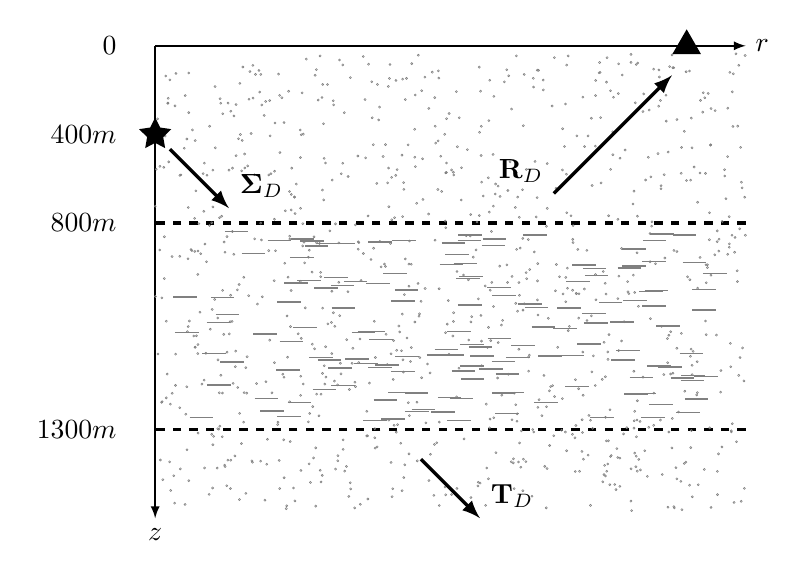
\begin{tikzpicture}[scale=0.75,line width=1.25]
		\def\l{10}
		\def\zs{1.5}
		\def\zb{3}
		\def\zN{6.5}
		\def\h{\zN+1.5}
		\def\r{9}
		\def\Nf{150}
		\def\Np{1000}
		\def\fraclen{.4}
		\draw[-latex,line width=.5] (0,\h) -- (0,0) node[below] {$z$};
		\node[left] at (0,\h) {$0\quad$};
		\draw[-latex,line width=.5] (0,\h) -- (\l,\h) node[right] {$r$};
		\draw[draw=none] (\l,\h-\zs) -- (0,\h-\zs) node[left] {$400m\quad$};
		\draw[dashed] (\l,\h-\zb) -- (0,\h-\zb) node[left] {$800m\quad$};
		\draw[dashed] (\l,\h-\zN) -- (0,\h-\zN) node[left] {$1300m\quad$};
		%\node[] (C) at (\l/2,{\h-\zN+(-\zb+\zN)/2}) {\Large$\vdots$};
		\node[] (C) at (\l/2,{\h-\zN+(-\zb+\zN)/2}){};
		\pgfmathsetseed{404}
		%fractures
		\foreach \i in {1,...,\Nf}{
			\pgfmathsetmacro\xi{(\l-1)*(rnd-.5)}
			\pgfmathsetmacro\yi{(\zN-\zb-.25)*(rnd-.5)}
				\draw[line width=.5,color=gray] (C) ++ (\xi,\yi) ++ (-\fraclen/2,0) --++ (\fraclen,0);
				}
		%pores \filldraw (0,0) circle (3pt);
		\foreach \i in {1,...,\Np}{
			\pgfmathsetmacro\xi{(\l)*(rnd-.5)}
			\pgfmathsetmacro\yi{(\h-.25)*(rnd-.5)}
				\draw[line width=0.2pt,gray,fill=none] (C) ++ (0,\zs/2) ++ (\xi,\yi) circle (0.5pt);
				}

		\node[star,star points=3,star point ratio=0.5,draw,fill=white,fill=black,rotate=180] (R) at (\r,\h) {};
		\node[star,star points=5,star point ratio=0.5,draw,fill=white,fill=black,rotate=180] (S) at (0,\h-\zs) {};
		
		\draw[-latex] (S) ++(.25,-.25) --++ (1,-1) node [anchor=south west] {$\boldsymbol{\Sigma}_D$};
		%\draw[-latex] (S) ++(.25,.25) --++ (1,1) node [anchor=north west] {$\boldsymbol{\Sigma}_U$};
		\draw[latex-] (R) ++(-.25,-.5) --++ (-2,-2) node [anchor=south east] {$\mathbf{R}_D$};
		\draw[-latex] (S) ++(\l/2-.5,-\h-.5) --++ (1,-1) node [anchor=south west] {$\mathbf{T}_D$};
		%\node[anchor=south] at (\l-.5,\h-\zN) {$\rho^{(k)},c_{ij}^{(k)}$};
	\end{tikzpicture}
\end{frame}
%------------------------------------------------
\begin{frame}{Reflection coefficients}\Large\centering
	\includegraphics<1>[width=.29\textwidth]{./Fig/rPP20}%
	\includegraphics<2>[width=.29\textwidth]{./Fig/rPP40}%
	\includegraphics<3>[width=.29\textwidth]{./Fig/rPP60}%
	\quad%
	\includegraphics<1>[width=.29\textwidth]{./Fig/rPS20}%
	\includegraphics<2>[width=.29\textwidth]{./Fig/rPS40}%
	\includegraphics<3>[width=.29\textwidth]{./Fig/rPS60}%
	\quad%	
	\includegraphics<1>[width=.29\textwidth]{./Fig/rSS20}%
	\includegraphics<2>[width=.29\textwidth]{./Fig/rSS40}%
	\includegraphics<3>[width=.29\textwidth]{./Fig/rSS60}%
\end{frame}
%------------------------------------------------
\begin{frame}{Common-shot gathers @ 50 Hz}\Large\centering
	\includegraphics<1>[width=.45\textwidth]{./Fig/CSG-Z1}%
	\includegraphics<1>[width=.45\textwidth]{./Fig/CSG-R1}%
	\includegraphics<2>[width=.45\textwidth]{./Fig/CSG-Z2}%
	\includegraphics<2>[width=.45\textwidth]{./Fig/CSG-R2}%
	\includegraphics<3>[width=.45\textwidth]{./Fig/CSG-Z3}%
	\includegraphics<3>[width=.45\textwidth]{./Fig/CSG-R3}%
	\includegraphics<4>[width=.45\textwidth]{./Fig/CSG-Z4}%
	\includegraphics<4>[width=.45\textwidth]{./Fig/CSG-R4}%
%	\includegraphics<5>[width=.45\textwidth]{./Fig/CSG-Z5}%
%	\includegraphics<5>[width=.45\textwidth]{./Fig/CSG-R5}%
%	\includegraphics<6>[width=.45\textwidth]{./Fig/CSG-Z6}%
%	\includegraphics<6>[width=.45\textwidth]{./Fig/CSG-R6}%
%	\includegraphics<7>[width=.45\textwidth]{./Fig/CSG-Z7}%
%	\includegraphics<7>[width=.45\textwidth]{./Fig/CSG-R7}%
	\includegraphics<5>[width=.45\textwidth]{./Fig/CSG-Z8}%
	\includegraphics<5>[width=.45\textwidth]{./Fig/CSG-R8}%
%	\includegraphics<9>[width=.45\textwidth]{./Fig/CSG-Z9}%
%	\includegraphics<9>[width=.45\textwidth]{./Fig/CSG-R9}%
	\includegraphics<6>[width=.45\textwidth]{./Fig/CSG-Z10}%
	\includegraphics<6>[width=.45\textwidth]{./Fig/CSG-R10}%
%	\includegraphics<11>[width=.45\textwidth]{./Fig/CSG-Z11}%
%	\includegraphics<11>[width=.45\textwidth]{./Fig/CSG-R11}%
%	\includegraphics<12>[width=.45\textwidth]{./Fig/CSG-Z12}%
%	\includegraphics<12>[width=.45\textwidth]{./Fig/CSG-R12}%
%	\includegraphics<13>[width=.45\textwidth]{./Fig/CSG-Z13}%
%	\includegraphics<13>[width=.45\textwidth]{./Fig/CSG-R13}%
	\includegraphics<7>[width=.45\textwidth]{./Fig/CSG-Z14}%
	\includegraphics<7>[width=.45\textwidth]{./Fig/CSG-R14}%
%	\includegraphics<15>[width=.45\textwidth]{./Fig/CSG-Z15}%
%	\includegraphics<15>[width=.45\textwidth]{./Fig/CSG-R15}%
%	\includegraphics<16>[width=.45\textwidth]{./Fig/CSG-Z16}%
%	\includegraphics<16>[width=.45\textwidth]{./Fig/CSG-R16}%
\end{frame}
%------------------------------------------------
\begin{frame}{CSG differences}\Large\centering
	\includegraphics<1>[width=.45\textwidth]{./Fig/diff-Z100200}%
	\includegraphics<1>[width=.45\textwidth]{./Fig/diff-R100200}%
	\includegraphics<2>[width=.45\textwidth]{./Fig/diff-Z200300}%
	\includegraphics<2>[width=.45\textwidth]{./Fig/diff-R200300}%
	\includegraphics<3>[width=.45\textwidth]{./Fig/diff-Z100300}%
	\includegraphics<3>[width=.45\textwidth]{./Fig/diff-R100300}%
\end{frame}
%------------------------------------------------
\begin{frame}{Traces at $x$ = 1 km}\Large\centering
	\includegraphics<1>[width=.85\textwidth]{./Fig/traces-Z}%
	\includegraphics<2>[width=.85\textwidth]{./Fig/traces-R}%
	\includegraphics<3>[width=.85\textwidth]{./Fig/tracesLate-Z}%
	\includegraphics<4>[width=.85\textwidth]{./Fig/tracesLate-R}%
\end{frame}
%------------------------------------------------
\begin{frame}{Fractured porous finely-layered media}
\centering
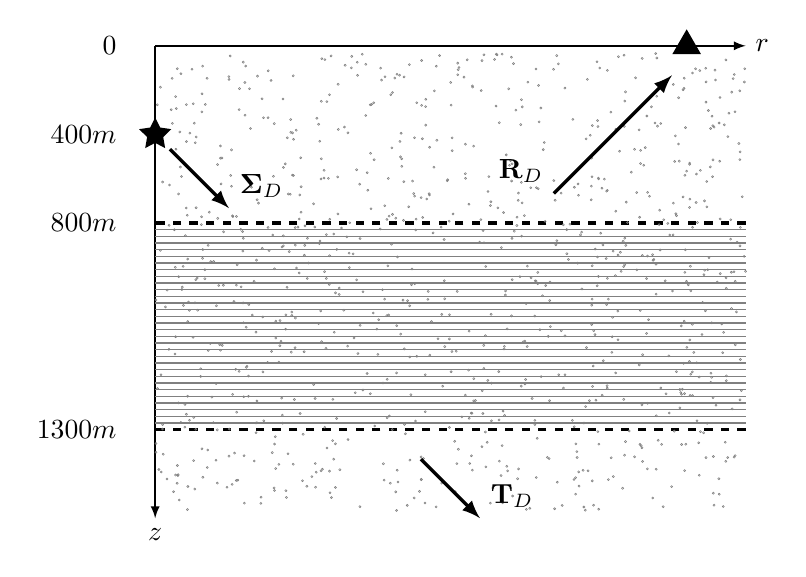
\begin{tikzpicture}[scale=0.75,line width=1.25]
		\def\l{10}
		\def\zs{1.5}
		\def\zb{3}
		\def\zN{6.5}
		\def\h{\zN+1.5}
		\def\r{9}
		\def\Nf{150}
		\def\Np{1000}
		\def\fraclen{.4}
		\draw[-latex,line width=.5] (0,\h) -- (0,0) node[below] {$z$};
		\node[left] at (0,\h) {$0\quad$};
		\draw[-latex,line width=.5] (0,\h) -- (\l,\h) node[right] {$r$};
		\draw[draw=none] (\l,\h-\zs) -- (0,\h-\zs) node[left] {$400m\quad$};
		\draw[dashed] (\l,\h-\zb) -- (0,\h-\zb) node[left] {$800m\quad$};
		\draw[dashed] (\l,\h-\zN) -- (0,\h-\zN) node[left] {$1300m\quad$};
		%\node[] (C) at (\l/2,{\h-\zN+(-\zb+\zN)/2}) {\Large$\vdots$};
		\node[] (C) at (\l/2,{\h-\zN+(-\zb+\zN)/2}){};
		
		\def\Nl{30}
		\foreach \i in {1,...,\Nl}{
			\pgfmathsetmacro\d{\i*(\zN-\zb)/(\Nl+1)}
			\draw[line width=.5,color=gray] (\l,{\h-\zb - \d}) -- (0,{\h-\zb - \d});
		}
		
%		\pgfmathsetseed{404}
%		%fractures
%		\foreach \i in {1,...,\Nf}{
%			\pgfmathsetmacro\xi{(\l-1)*(rnd-.5)}
%			\pgfmathsetmacro\yi{(\zN-\zb-.25)*(rnd-.5)}
%				\draw[line width=.5,color=gray] (C) ++ (\xi,\yi) ++ (-\fraclen/2,0) --++ (\fraclen,0);
%				}

		%pores
		\foreach \i in {1,...,\Np}{
			\pgfmathsetmacro\xi{(\l)*(rnd-.5)}
			\pgfmathsetmacro\yi{(\h-.25)*(rnd-.5)}
				\draw[line width=0.2pt,gray,fill=none] (C) ++ (0,\zs/2) ++ (\xi,\yi) circle (0.5pt);
				}

		\node[star,star points=3,star point ratio=0.5,draw,fill=white,fill=black,rotate=180] (R) at (\r,\h) {};
		\node[star,star points=5,star point ratio=0.5,draw,fill=white,fill=black,rotate=180] (S) at (0,\h-\zs) {};
		
		\draw[-latex] (S) ++(.25,-.25) --++ (1,-1) node [anchor=south west] {$\boldsymbol{\Sigma}_D$};
		%\draw[-latex] (S) ++(.25,.25) --++ (1,1) node [anchor=north west] {$\boldsymbol{\Sigma}_U$};
		\draw[latex-] (R) ++(-.25,-.5) --++ (-2,-2) node [anchor=south east] {$\mathbf{R}_D$};
		\draw[-latex] (S) ++(\l/2-.5,-\h-.5) --++ (1,-1) node [anchor=south west] {$\mathbf{T}_D$};
		%\node[anchor=south] at (\l-.5,\h-\zN) {$\rho^{(k)},c_{ij}^{(k)}$};
	\end{tikzpicture}
\end{frame}
%------------------------------------------------
\begin{frame}{Reflection coefficients}\Large\centering
	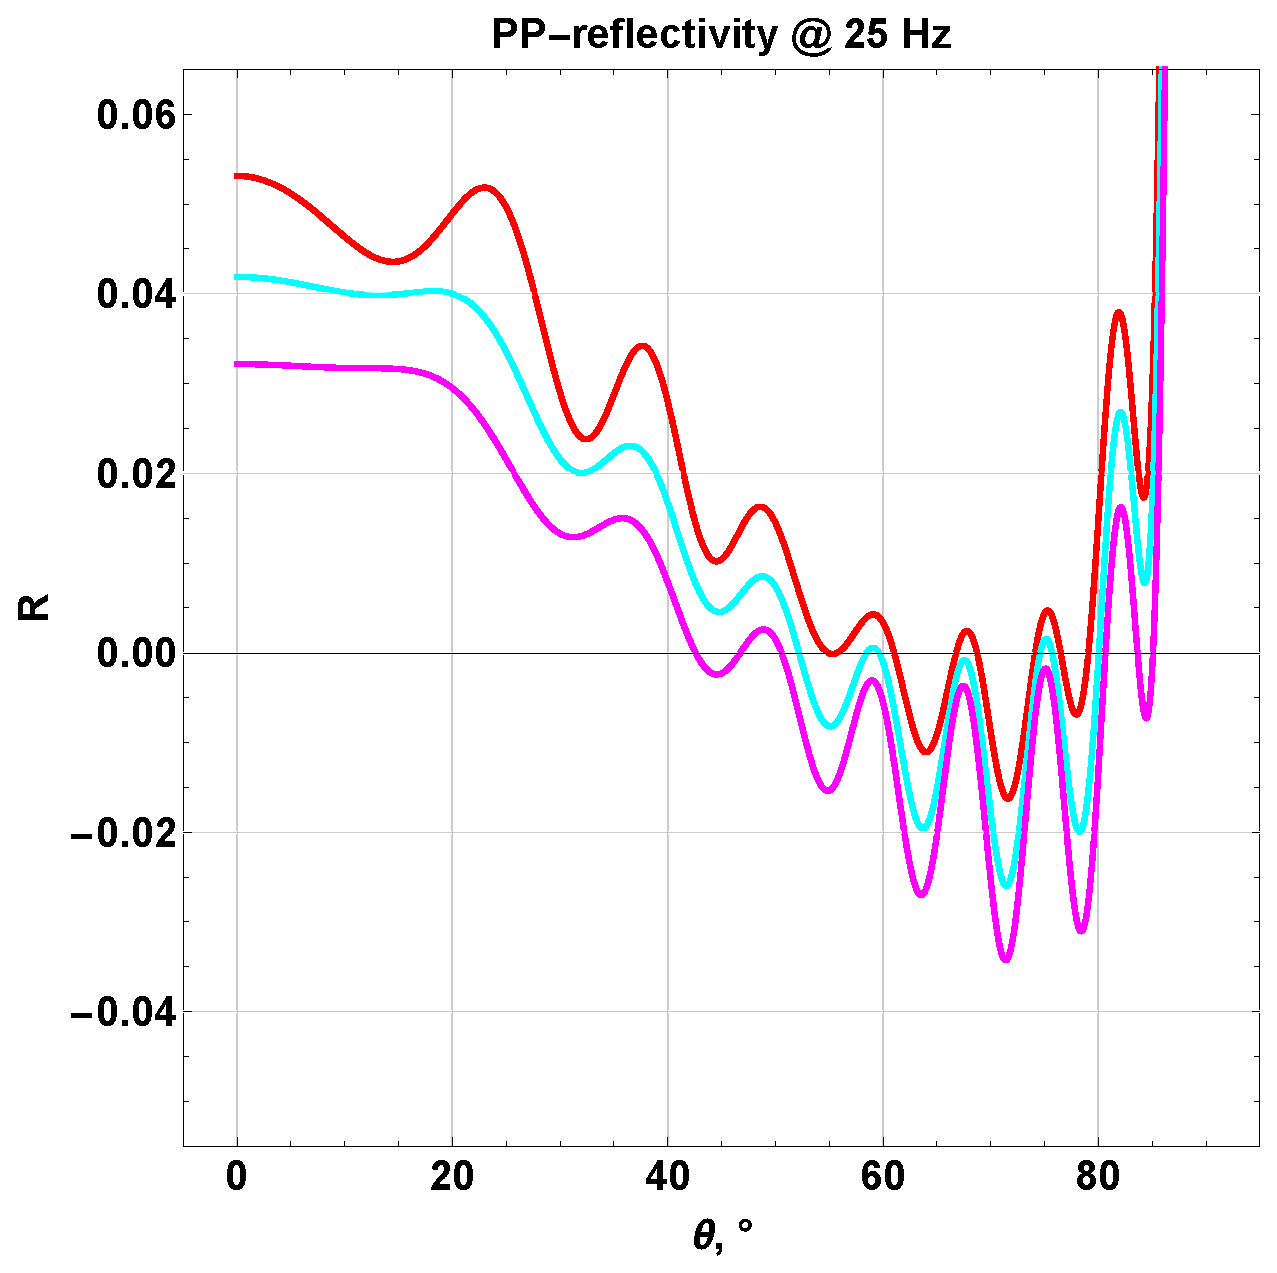
\includegraphics[width=.29\textwidth]{./Fig/respPP25}%
	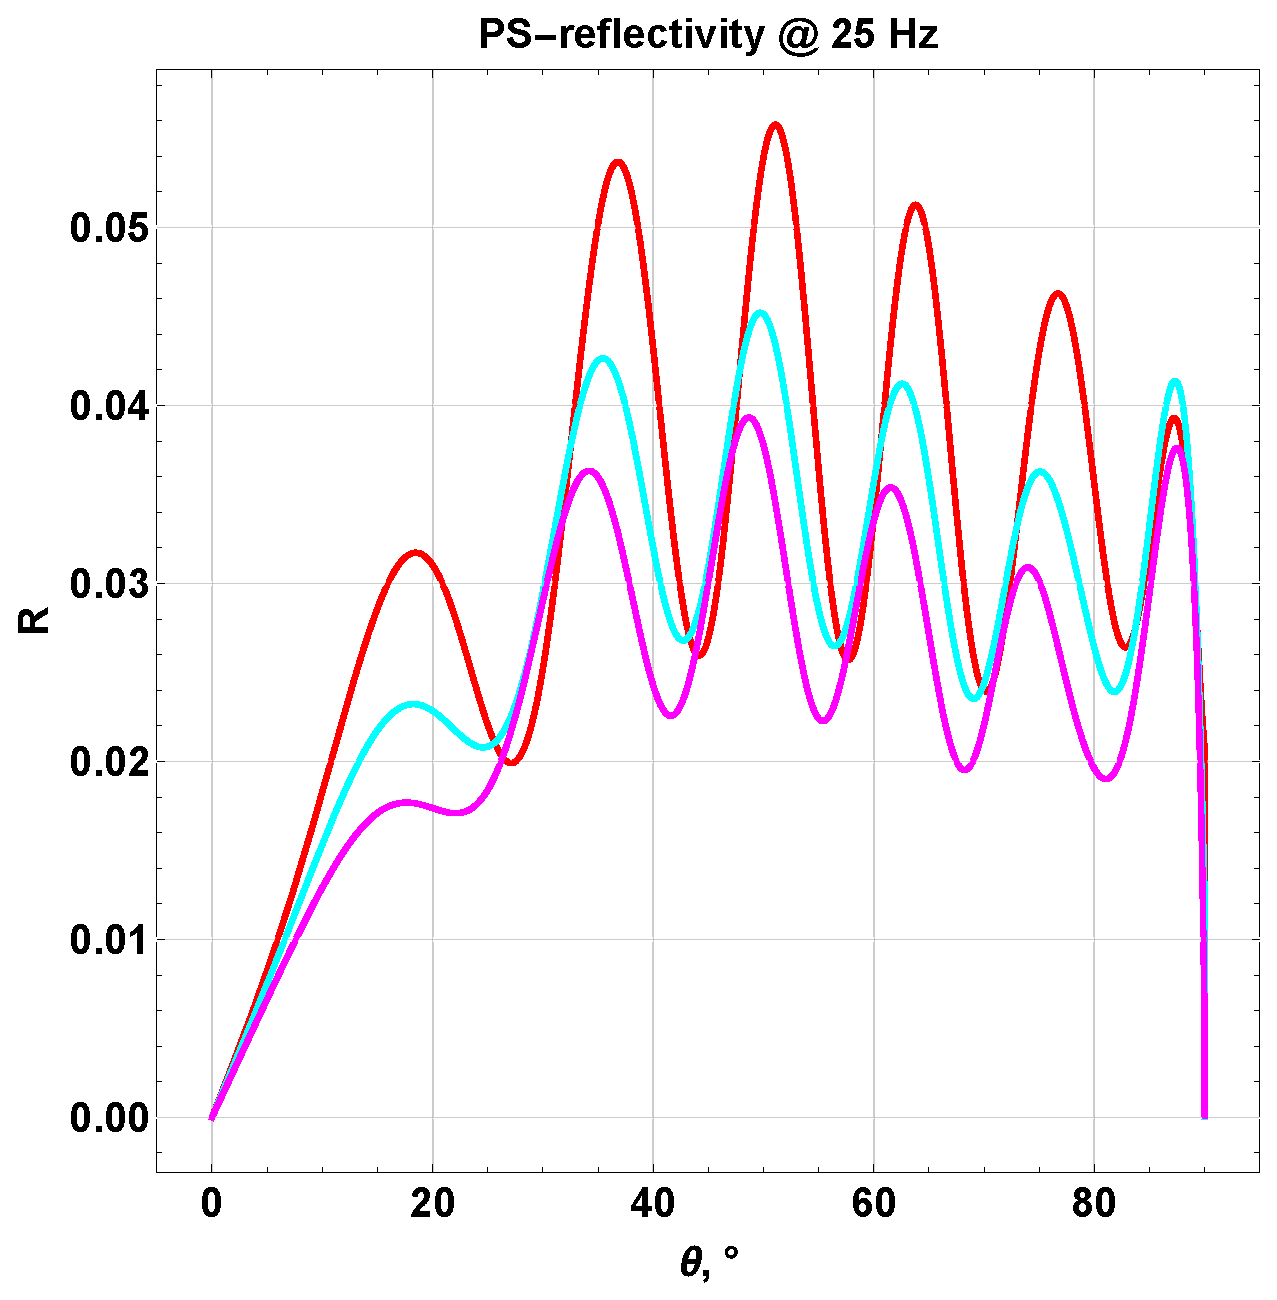
\includegraphics[width=.29\textwidth]{./Fig/respPS25}%
	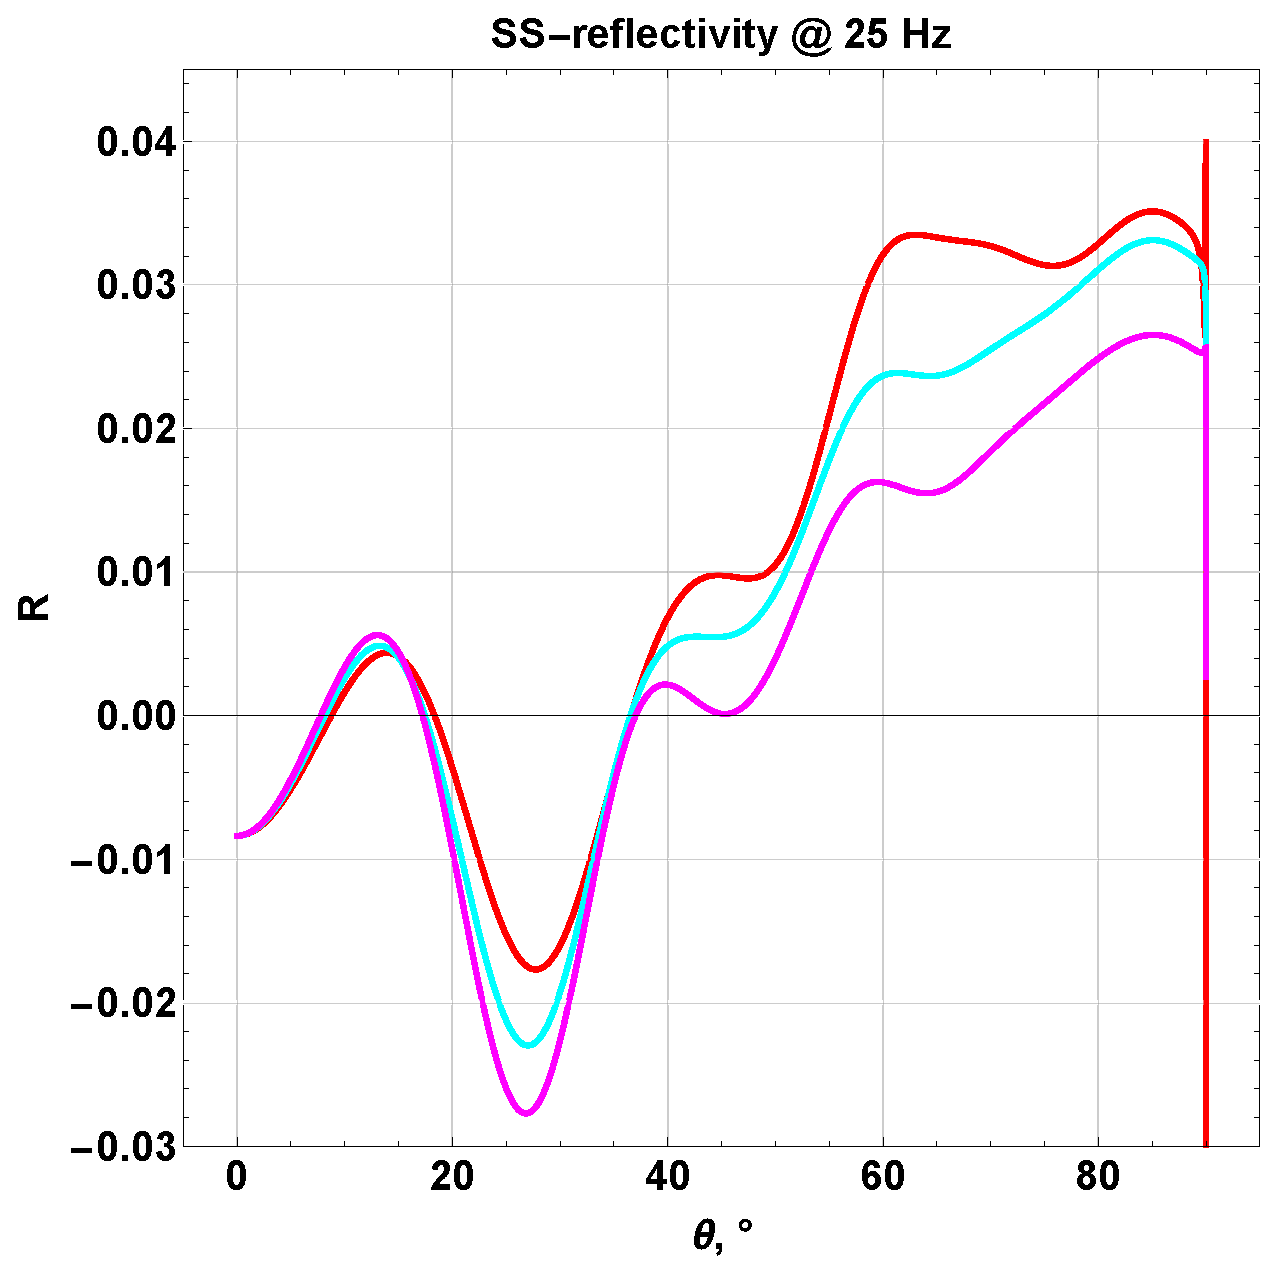
\includegraphics[width=.29\textwidth]{./Fig/respSS25}%
\end{frame}
%------------------------------------------------
\begin{frame}{Common-shot gathers @ 25 Hz}\Large\centering
	\includegraphics<1>[width=.45\textwidth]{./Fig/CSGN25-Z1}%
	\includegraphics<1>[width=.45\textwidth]{./Fig/CSGN25-R1}%
	\includegraphics<2>[width=.45\textwidth]{./Fig/CSGN25-Z2}%
	\includegraphics<2>[width=.45\textwidth]{./Fig/CSGN25-R2}%
\end{frame}
%------------------------------------------------
\begin{frame}{Thin lamination}\Large\centering
	\includegraphics<1>[width=.85\textwidth]{./Fig/traces25-Z}%
	\includegraphics<2>[width=.85\textwidth]{./Fig/traces25-R}%
\end{frame}
%------------------------------------------------
\section{Discussion \& Conclusions}
%------------------------------------------------
\begin{frame}{Discussion \& Conclusions}
\setbeamertemplate{itemize items}[triangle]\large
\begin{itemize}
	\item Reflectivity modelling. Practical albeit limited approach for complex models:
		\begin{itemize}
			\item[$+$] Low-symmetry anisotropic frequency-dependent models,
			\item[$+$] Partial response (e.g., PP-reflection),
			\item[$+$] Source waveform independent,
			\item[$+$] Multiple source formulations (e.g., force, moment tensor),
			\item[$-$] Effective models,
			\item[$-$] Flat layers.
		\end{itemize}\pause
	\item Rock-physics model. Simple yet realistic:
		\begin{itemize}
			\item[$+$] Multiple-scale inclusions,
			\item[$+$] Multiple fluids,
			\item[$+$] Calibrated to real rocks,
			\item[$-$] No fracture interaction.
		\end{itemize}
\end{itemize}
\end{frame}
%------------------------------------------------
\begin{frame}{Discussion \& Conclusions}
\setbeamertemplate{itemize items}[triangle]\large
\begin{itemize}
	\item Modelling results. 
		\begin{itemize}
			\item[$+$] Fracture effects in seismic frequency band,
			\item[$+$] Phase and amplitude effects,
			\item[$+$] Can be confused with thin-bedding.
			\item[$-$] Difficult to interpret.
		\end{itemize}\pause
	\item Future research (besides more detailed analysis):
		\begin{itemize}
			\item[$\rightarrow$] Inversion for fracture parameters,
			\item[$\rightarrow$] Vertical fractures,
			\item[$\rightarrow$] Multiple fracture sets,
			\item[$\rightarrow$] Code release.
		\end{itemize}
\end{itemize}
\end{frame}
%------------------------------------------------

\begin{frame}{References}
\centering
\bibliographystyle{seg}
\bibliography{../../../../../Latex/References}
\end{frame}

%----------------------------------------------------------------------------------------
\end{document} 
%
%
%
%
%
%
%
%
%
%
%
%
%
%
%
%
%